 % \vspace{-0.5em}
\section{Experiments}
 % \vspace{-0.5em}


\subsection{Setups}\label{sec:setup}

% \vspace{0.1em}
\textbf{Datasets and models.} For the fine-tuning setting,
we select $416 / 417$ samples on Pokémon~\cite{Pokemon-Blip}, $2500 / 2500$ samples on MS-COCO \cite{lin2014microsoft} and $10,000 / 10,000$ samples on Flickr \cite{young2014image} as the member/hold-out dataset, respectively. These three datasets involve diverse data distributions and dataset scales.
We use the most widely used text-to-image diffusion model, Stable Diffusion v1-4\footnote{ \url{https://huggingface.co/CompVis/stable-diffusion-v1-4}}~\cite{Stable-Diffusion-v1-4}, as the target model to fine-tune it on these three datasets. 
For the pretraining setting,
we conduct experiments on Stable Diffusion v1-5\footnote{\url{https://huggingface.co/runwayml/stable-diffusion-v1-5}}~\cite{Stable-Diffusion-v1-5} using the processed LAION dataset~\cite{schuhmann2022laion} (detailed in Sec.~\ref{sec:main_result}) to minimize distribution shift~\cite{dubinski2024towards,das2024blind}.

% \vspace{0.1em}
\textbf{Fine-tuning setups.}
For fine-tuning, previous membership inference on text-to-image diffusion models usually relies on strong overfitting settings. To evaluate the performance more realistically, we consider the two following setups: (1) \textit{Over-training.} Following the previous works~\cite{duan2023diffusion, kong2023efficient, fu2023probabilistic}, we fine-tune 15,000 steps on Pokemon datasets, and 150,000 steps on MS-COCO and Flickr (with only $2500 / 2500$ dataset size). (2) \textit{Real-world training.}  Considering that trainers typically do not train for such high steps, we recalibrate the steps based on the 
training steps/dataset size ratio (approximately 20) of official fine-tuning scripts on Huggingface~\cite{text-to-image-ft}. Thus, we train 7,500 steps, 50,000 steps and 200,000 steps for the Pokémon, MS-COCO and Flickr datasets, respectively. Additionally, we employ the default data augmentation (Random-Crop and Random-Flip~\cite{text-to-image-ft-python}) in training codes \cite{text-to-image-ft-python} to simulate real-world scenarios.





% \vspace{0.1em}
\textbf{Baselines.} We broadly consider existing member inference methods applicable to text-to-image diffusion models as our baselines: Loss-based inference~\cite{matsumoto2023membership}, SecMI$ _\text{stats} $ (SecMI)~\cite{duan2023diffusion}, PIA~\cite{kong2023efficient},  PFAMI$ _\text{Met} $ (PFAMI)~\cite{fu2023probabilistic} and an additional method of directly conducting Monte Carlo estimation (M. C.) on Eq.~\eqref{eq:elbo_loss} for comparison. For all baselines, we use the parameters recommended in their papers.
We omit some membership inference methods for generative models \cite{liu2019performing, chen2020gan, hayes2019logan}, as they have been shown ineffective for diffusion models in previous works \cite{duan2023diffusion, fu2023probabilistic}.  

% \vspace{0.1em}
\textbf{Evaluation metrics.}  
We follow the widely used metrics of previous works \cite{carlini2022membership,carlini2023extracting, duan2023diffusion, kong2023efficient, fu2023probabilistic}, including ASR (i.e., the accuracy of membership inference), AUC and the True Positive Rate (TPR) when the False Positive Rate (FPR) is 1\% (i.e.,  TPR@1\%FPR). 

% \vspace{0.1em}
\textbf{Implementation details.}
Our evaluation follows the setup of representative membership inference works  \cite{carlini2022membership, carlini2023extracting}. 
It is important to note that some implementations \cite{sec_implement, pia_implement} of previous works assume access to a portion of the exact member set and the hold-out set to obtain a threshold for calculating ASR or to train a classification network \cite{sec_implement}. This assumption does not align with real-world scenarios. 
Therefore, we strictly adhere to the fundamental assumption of membership inference \cite{carlini2022membership, fu2023probabilistic}: knowing only the overall dataset without any knowledge of the member/hold-out split. Hence, we first train a shadow model to obtain the 
$\alpha$ for Eq.~\eqref{eq:mi_th}, classifiers for Eq.~\eqref{eq:mi_vec}  and the threshold $\tau$ for 
calculating ASR with auxiliary datasets of the same distribution. Then we perform the test on the target models.
Other implementation details are provided in Appendix~\ref{appd:detail}.

\vspace{-7pt}
\subsection{Main Results}
\vspace{-3pt}

\label{sec:main_result}
\begin{table}[tbp]
  \centering
  \caption{Results under \textit{Over-training} setting. We mark the best and second-best results for each metric in \textbf{bold} and \underline{underline}, respectively. Additionally, the best results from baselines are marked in \blue{blue} for comparison.}
  \footnotesize
  \resizebox{\linewidth}{!}
  {
       \begin{threeparttable}
 \begin{tabular}{l ccc ccc ccc c}
    \toprule
    \multirow{2}[2]{*}{Method} & \multicolumn{3}{c}{MS-COCO} & \multicolumn{3}{c}{Flickr} & \multicolumn{3}{c}{Pokemon} & \multirow{2}[2]{*}{Query} \\
    \cmidrule(lr){2-4} 
    \cmidrule(lr){5-7}
    \cmidrule(lr){8-10}
          & ASR   & AUC   & TPR@1\%FPR   & ASR   & AUC   & TPR@1\%FPR & ASR   & AUC   & TPR@1\%FPR &  \\
    \midrule
    Loss
    & 81.92 & 89.98	& 32.28
    &81.90	&90.34	&40.80
   &83.76	&91.79	&25.77 
    & 1 \\
    PIA   & 68.56 & 75.12 & 5.08  
    &   68.56    &  75.12     &   5.08    
    & 83.37 & 90.95 & 13.31 
    & 2 \\
    M. C. 
    & 82.04 & 89.77 & 36.04
    & 83.32 & 91.37 & 41.20 
    & 79.35 & 86.78 & 23.74
    & 3 \\
    SecMI 
     &  83.00     & 90.81      &     50.64
    & 62.96$^\dagger$ & 89.29 & 48.52
    & 80.49 & 90.64 & 9.36  
    & 12 \\
    
     PFAMI 
    &\blue{94.48}	&\blue{98.60}	&\blue{78.00}
    &\blue{90.64}	&\blue{96.78}	&\blue{50.96}
    &\blue{89.86}	&\blue{95.70}	&\blue{65.35}
    & 20 \\
    \midrule
    \clidth & \underline{99.08} & \textbf{99.94} & \textbf{99.12} 
    & \underline{91.42} & \underline{97.39} & \textbf{74.00} 
    & \textbf{97.96} & \underline{99.28} & \textbf{97.84} & 15 \\
    \clidvec & \textbf{99.74} & \underline{99.31} & \underline{95.20} 
    &\textbf{91.78} & \textbf{97.52} & \underline{73.88} 
    & \underline{97.36} & \textbf{99.46} & \underline{96.88} & 15 \\
     \bottomrule
    \end{tabular}%
    \begin{tablenotes}
        \item $^\dagger$ When conducting SecMI~\cite{duan2023diffusion},  we observe that the thresholds obtained on the shadow model sometimes do not transfer well to the target model.
    \end{tablenotes}
    \end{threeparttable}
    \label{table:results_over}
    }
\end{table}%

\begin{table}[tbp]
    \vspace{-7pt}
  \centering
  \caption{Results under \textit{Real-world training} setting. We also highlight key results according to Tab.~\ref{table:results_over}.}
  \footnotesize
  \resizebox{\linewidth}{!}
  {
    \begin{tabular}{l ccc ccc ccc c}
    \toprule
    \multirow{2}[2]{*}{Method} & \multicolumn{3}{c}{MS-COCO} & \multicolumn{3}{c}{Flickr} & \multicolumn{3}{c}{Pokemon} & \multirow{2}[2]{*}{Query} \\
    \cmidrule(lr){2-4} 
    \cmidrule(lr){5-7}
    \cmidrule(lr){8-10}
          & ASR & AUC   & TPR@1\%FPR & ASR   & AUC   & TPR@1\%FPR & ASR   & AUC   & TPR@1\%FPR &  \\
    \midrule
    Loss
   & 56.28 &	61.89&	1.92
    &54.91	&56.60	&1.83
    &61.03	&65.96	&2.82 
    & 1 \\
     PIA   & 54.10 & 55.52 & 1.76  & 51.96 & 52.73 & 1.28  & 58.34 & 59.95 & 2.64  & 2 \\
    M. C. & 57.98 & 61.97 & 2.64  & 54.92 & 56.78 & 2.16  & 61.10 & \blue{66.48} & 3.84  
    & 3 \\
    SecMI & \blue{60.94} & \blue{65.40} & \blue{3.92}
    & \blue{55.60} & \blue{63.85} & \blue{2.76}  
    & \blue{61.28} & 65.56 & 0.84  
    & 12 \\
   
     PFAMI
    &57.36	&60.39	&2.72
    &54.68	&56.13	&1.80
    &58.94	&63.53	&\blue{5.76}
    & 20 \\
    \midrule
    \clidth 
    & \underline{88.88} & \underline{96.13} & \textbf{67.52} 
    & \underline{87.12} & \underline{94.74} & \underline{53.56} & \textbf{86.79} 
    & \textbf{93.28} & \textbf{61.39} 
    & 15 \\
    \clidvec 
    & \textbf{89.52} & \textbf{96.30} & \underline{66.36} 
    & \textbf{88.86} & \textbf{95.33} & \textbf{53.92} 
    & \underline{85.47} & \underline{92.61} & \underline{59.95} 
    & 15 \\
    \bottomrule
    \end{tabular}%
    \label{table:results_real}
    }
    \vspace{-9pt}
\end{table}%


% \vspace{0.10cm}
\textbf{Over-training setting (fine-tuning).}
In Tab.~\ref{table:results_over}, models are trained for excessive steps on all three datasets, resulting in significant overfitting. We observe that under this over-training scenario, both of our methods nearly achieve ideal binary classification effectiveness. For instance, \clidth achieves over 99\% ASR, AUC and TPR@1\%FPR value on the MS-COCO dataset \cite{lin2014microsoft}.
With this training setup, the metrics for different baselines are very similar.  
Even the simplest loss-based method \cite{matsumoto2023membership} (with the query count of 1) also yields satisfactory results compared with other high query count methods.
Therefore, we emphasize: \textit{This unrealistic over-training setting fails to adequately reflect the effectiveness differences among various membership inference methods}.


% \vspace{0.10cm}
\textbf{Real-world training setting (fine-tuning).}
In Tab.~\ref{table:results_real}, we adjust the training steps simulating real-word training scenario \cite{text-to-image-ft} and utilize default data augmentation \cite{text-to-image-ft-python}. The best value of ASR and AUC of baseline methods decreases to around 65\%, and the best value of TPR@1\%FPR decreases to around 5\%, indicating insufficient effectiveness of previous member inference methods in real-world training scenarios of text-to-image diffusion models. 
In contrast, our methods maintain ASR above 86\% and AUC above 93\%,  exceeding the best baseline values by about 30\%. The TPR@1\%FPR of our methods exceeds the best baseline values by  50\%\textasciitilde60\%.
The results demonstrate the effectiveness of our methods across various data distributions and scales in real-world training scenarios.



\textbf{Pretraining setting.}
For the pretraining setting, we adopt a stringent and realistic membership inference setting based on previous works~\cite{dubinski2024towards,das2024blind}. (1) To ensure the distribution consistency between the member and hold-out set, we respectively select $2500$ samples from the LAION-Aesthetics v2 5+ and LAION-2B MultiTranslated \cite{schuhmann2022laion} as member/hold-out set following~\cite{dubinski2024towards}; (2) We filter out samples containing non-English characters to ensure there are no other "distinguishable tails"~\cite{das2024blind} in the dataset\footnote{\citet{das2024blind} indicates that MultiTranslated-LAION dataset contains fewer non-English characters than the LAION dataset due to the use of the translation model. }.
We conduct membership inference on Stable Diffusion v1-5~\cite{rombach2022high}. 
As shown in Tab.~\ref{tab:wrap_pretrain}, our method consistently outperforms the baselines across all three metrics. 

\begin{figure}[t]
\makeatletter\def\@captype{table}\makeatother
\begin{minipage}{0.45\linewidth}
\centering
\footnotesize
\resizebox{0.99\linewidth}{!} {
    \setlength{\tabcolsep}{5pt}
    \begin{tabular}{lccccccc}
    \toprule
    \multirow{2}[2]{*}{Method} &  \multicolumn{3}{c}{LAION} & \multirow{2}[2]{*}{Query} \\
  \cmidrule(lr){2-4}       & ASR   & AUC   & TPR@1\%FPR &  \\
    \midrule
    Loss      & 51.78 &	50.90 &	1.75
    & 1 \\
    PIA         & 52.13 & 52.42 & 1.25  & 2 \\
    M. C.        & 53.18 & 53.96 & 1.25  & 3 \\
    SecMI        & 57.43 & 58.59 & 2.45  & 12 \\
    PFAMI       & 59.08 & 61.11 &	1.45
    & 20 \\
    \midrule
    \clidth   & \textbf{64.53} & \textbf{67.82} & \textbf{5.01}  & 15 \\
    \bottomrule
    \end{tabular}%
}
% \vspace{1em}
\caption{The performance of membership inference methods on Stable Diffusion v1-5~\cite{Stable-Diffusion-v1-5} in pretraining setting. 
We utilize the processed LAION dataset to ensure the distribution consistency between member / hold-out sets~\cite{dubinski2024towards,das2024blind}.
The best results are highlighted in \textbf{bold}.}
  \label{tab:wrap_pretrain}%
\end{minipage}
\hspace{1ex}
%%%%%%%%%%%%%%%%%%%%%%%%%
\makeatletter\def\@captype{figure}\makeatother
\begin{minipage}{0.5\linewidth}
\centering
\vspace{-1em}
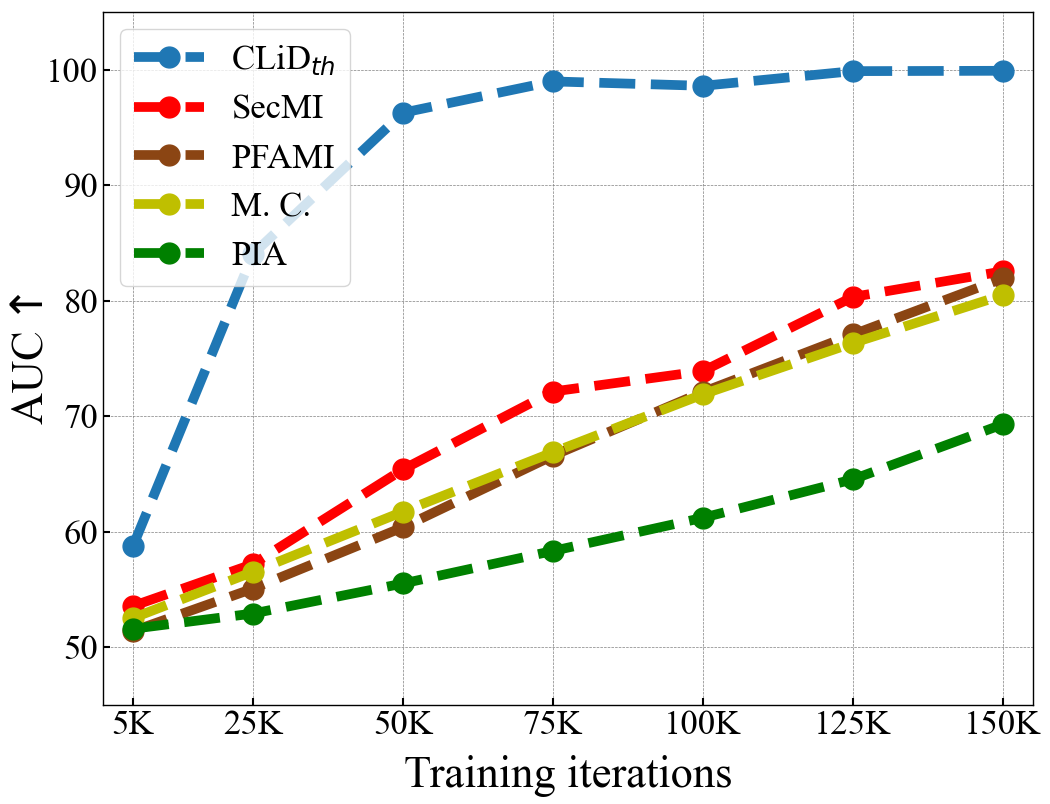
\includegraphics[scale=0.25]{imgs/auc_steps.png}
\vspace{-0.5em}
\caption{Effectiveness trajectory on various training steps. 
}
\label{fig:auc_steps}
\end{minipage}
\vspace{-9pt}
\end{figure}

\vspace{-2pt}
\subsection{Performance on Various Training Steps}
\vspace{-1pt}

\label{sec:vary_steps}
From Tab.~\ref{table:results_over} and Tab.~\ref{table:results_real}, we find that the training steps greatly influence the effectiveness of membership inference. 
All membership inference methods tend to exhibit satisfactory performance when the model is trained for an excessive number of steps that conflicts with real-world scenarios.
Therefore, we emphasize that the \textit{\textbf{effectiveness trajectory}} of membership inference across varying training steps should also be utilized to evaluate different methods. Better membership inference methods should reveal membership information earlier as training progresses.

 
To explore this, we fine-tune Stable Diffusion models with the MS-COCO dataset for varying training steps under \textit{real-world training} setting and report the AUC values of different membership inference methods in Fig.~\ref{fig:auc_steps}. 
It can be observed that as the training progresses, \clidth exhibits a significantly faster increase in effectiveness trajectory. By $25,000$ steps, \clidth effectively exposes membership information, whereas other baselines achieve similar results only at around $150,000$ steps. This demonstrates that our method can effectively reveal membership information when the overfitting degree of the text-to-image diffusion model is much weaker.


% \vspace{0.5cm}
\vspace{-2pt}
\subsection{Ablation Study} 
\vspace{-1pt}
% \vspace{-3pt}

\label{sec:ablation}

\begin{wrapfigure}[17]{r}{0.45\textwidth}
\centering
\vspace{-1.5em}
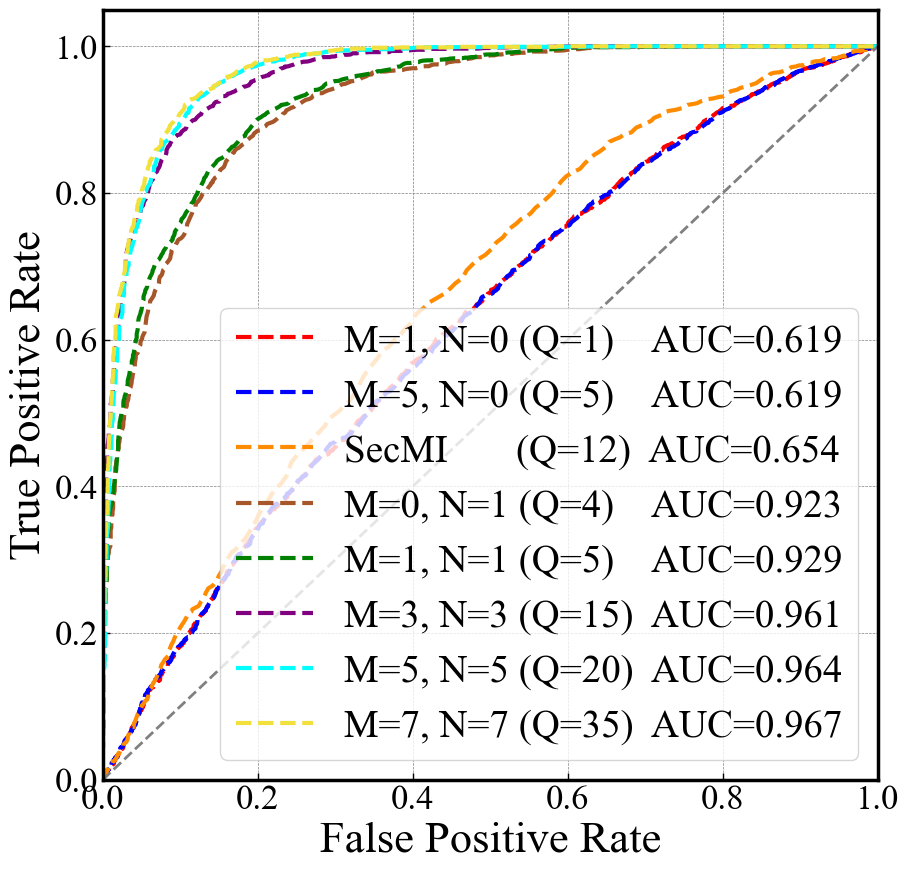
\includegraphics[scale=0.24]{imgs/auc_N_samples.png}
\vspace{-1em}
\caption{Performance of \clidth and SecMI under various Monte Carlo sampling numbers (i.e., query count). 
The legend labels are sorted in ascending order by AUC values.
}
\label{fig:auc_samples}
\end{wrapfigure}
To conduct an ablation study, we vary the Monte Carlo sampling count in  Eq.~\eqref{eq:clid_loss_reduction}  and Eq.~\eqref{eq:elbo_loss}, perform $\text{CLiD}_{th}$ with MS-COCO dataset under \textit{real-world training} setting and report the AUC values in Fig.~\ref{fig:auc_samples}.   
To further compare the effects of Eq.~\eqref{eq:clid_loss_reduction}  and Eq.~\eqref{eq:elbo_loss}, we discard each term in Eq.~\eqref{eq:mi_th} and denote it as $M / N=0$.
We also include the result of the best baseline, SecMI~\cite{duan2023diffusion}, as a comparison. 




\textbf{Effect of $ \mathcal{D}_{\mathbf{x},\mathbf{c},\mathbf{c}^*}$.} 
In Fig.~\ref{fig:auc_samples}, results of "M=1, N=0" and "M=1, N=1"  show a significant improvement of membership inference by including $ \mathcal{D}_{\mathbf{x},\mathbf{c},\mathbf{c}^*}$. Results of "M=5, N=0" and "M=1, N=1" further show that the method utilizing $\mathcal{D}_{\mathbf{x},\mathbf{c},\mathbf{c}^*}$ performs much better under the same sampling numbers. Additionally, the results of "M=0, N=1" and "M=1, N=1" indicates that only considering both Eq.~\eqref{eq:clid_loss_reduction} 
and Eq.~\eqref{eq:elbo_loss}  achieves the optimal performance. 


\textbf{Monte Carlo sampling numbers.} 
In Fig.~\ref{fig:auc_samples}, we observe that when setting $M=N$, the performance improves as the number of Monte Carlo sampling increases. And the performance is improved slightly when $M, N>3$. Hence, we set $M, N=3$ 
% in experiments (Sec.~\ref{sec:setup}) 
to ensure the balance between a low query count and satisfied performance. Moreover, the experiment results of "M=1, N=1" and "SecMI" also demonstrate: \clidth outperforms previous works even with a much fewer query count.


\begin{table}[t]
\setlength{\tabcolsep}{8pt}
    \centering
  \caption{The performance of different methods under no augmentation and default augmentation. }
  \footnotesize
  \resizebox{\linewidth}{!}
  {
    \begin{threeparttable}
    \begin{tabular}{lcccccc}
    \toprule
    \multirow{2}[2]{*}{Method} 
          & \multicolumn{3}{c}{No Augmentation } & \multicolumn{3}{c}{Defaut Augmentation } \\
\cmidrule(lr){2-4}  \cmidrule(l){5-7}        & \multicolumn{1}{c}{ASR} & \multicolumn{1}{c}{AUC} & \multicolumn{1}{c}{TPR@1\%FPR} & \multicolumn{1}{c}{ASR ($\Delta$)} & \multicolumn{1}{c}{AUC ($\Delta$)} & \multicolumn{1}{l}{TPR@1\%FPR ($\Delta$)} \\
    \midrule
    Loss  
    & 66.54 &	72.73& 	7.72 
    &   56.28 (-10.26) &	61.89 (-10.84)& 	1.92 (-5.80) 
\\
 \textcolor{gray}{PIA}$^\dagger$  & \textcolor{gray}{56.56} &	\textcolor{gray}{59.28} &	\textcolor{gray}{2.00}
       &  \textcolor{gray}{54.10~(-2.46)} &	\textcolor{gray}{55.52~(-3.76)} &	\textcolor{gray}{1.76~(-0.24)}
 \\
    % M. C.  
    % &       &       &      
    % &       &       &  \\
    SecMI &   72.02	&81.07	&13.72
    &    60.94 (-11.08)   &   65.40 (-15.08)    &3.92 (-9.80)  \\
   
     PFAMI  &  79.20 & 	87.05& 	18.44 
      &  57.36 (-21.84)     & 60.39 (-26.66)      &2.72 (-15.72)  \\
    \midrule
    \clidth &  96.76 &	99.47 &	91.72
       &   88.88 \textbf{(-7.88)}    & 96.13 \textbf{(-3.34)}      &67.52 (-24.20)$^\ddagger$ \\
    \bottomrule
    \end{tabular}%
\begin{tablenotes}
    \item 
    $^\dagger$We omit the discussion of PIA as it shows no effectiveness at this training steps, with the metrics consistently approximating random guessing.
    \vspace{0.1cm}
    \item
    $^\ddagger$The TPR@1\%FPR value changes significantly here because its ROC curve is very sharp when FPR close to $0$.
    \end{tablenotes}
    \end{threeparttable}
    \label{tab:aug_defense}
    }
    \vspace{-1em}
\end{table}%

% \vskip 2em
\begin{wraptable}{r}{0.45\textwidth}
\setlength{\tabcolsep}{2.5pt}
  \centering
    % \scriptsize
  \vspace{-1.75em}
   \caption{Effectiveness of \clidth in adaptive defense. We calculate the FID \cite{heusel2017gans} with $10,000$ unseen MS-COCO samples to assess the model utility.}
   \vspace{0.5em}
      \resizebox{\linewidth}{!}
  {
      \begin{threeparttable}
   \begin{tabular}{lcccc}
    \toprule
    \multicolumn{1}{c}{\multirow{2}[2]{*}{Defense}} & \multicolumn{3}{c}{\clidth on MS-COCO} &  \multirow{2}[2]{*}{ FID $\downarrow$ / \textcolor{blue}{$\Delta$}} \\
\cmidrule{2-4}          & ASR   & AUC   & TPR@1\%FPR   \\
    \midrule
    None &88.88 	&96.13 &	67.52 
   & 13.17  \\
    \midrule
    Reph & 85.32 &	93.83 &	55.67      
    & 13.58 / \textcolor{blue}{+0.41} \\
    Del-1 & 86.40 &	93.59 &	59.52 
    & 13.18 / \textcolor{blue}{-0.01} \\
    Del-3 & 83.91 &	91.52 &	52.03 
    & 12.92 / \textcolor{blue}{-0.25} \\
    Shuffle & \textcolor{gray}{65.89} & \textcolor{gray}{67.37} & \textcolor{gray}{0.15}  & \textcolor{gray}{18.26 /  \textcolor{red}{+5.09}}$^\dagger$ \\
    \bottomrule
    \end{tabular}%
    \begin{tablenotes}
    \item
    $^\dagger$Compared to other methods, the increase in FID caused by shuffling is unacceptable for generative models.
    \end{tablenotes}
    \end{threeparttable}
  \label{tab:adaptive}%
  }
    \vspace{-0.4em}
\end{wraptable}
\vspace{-3pt}
\subsection{Resistance to Defense}\label{sec:defense}
\vspace{-3pt}

Since data augmentation is commonly used in training and can mitigate the effectiveness of membership inference~\cite{duan2023diffusion}, we use it to evaluate the performance 
 of methods under defense. 
As the baseline methods already exhibit weak performance under \textit{real-world training} setting, we opt not to incorporate additional data augmentation. Instead, we remove the default data augmentation from training scripts \cite{text-to-image-ft-python} to observe the effectiveness change of different methods. We fine-tune Stable Diffusion models for 50,000 steps with MS-COCO, report the metrics, and calculate the metrics changes in Tab.~\ref{tab:aug_defense}. 
We observe that the effectiveness of all membership inference methods declines after data augmentation is introduced during training. 
Note that PFAMI~\cite{fu2023probabilistic} exhibits the highest sensitivity to data augmentation since it infers membership by probability fluctuation after images are perturbed, which also explains its significant performance decline between Tab.~\ref{table:results_over} and Tab.~\ref{table:results_real}.
Compared to the baselines, our method exhibits the smallest decrease, which indicates its stronger resistance to data augmentation. 

\textbf{Adaptive defense.} 
We further consider adaptive defense: assuming the trainers are aware of our methods and perturb the text of image-text datasets before training. We consider the following adaptive defense methods: (1) rephrasing the original text\footnote{We utilize ChatGPT-3.5 with the following prompt: "Please rewrite the following sentences while keeping the key semantics."}, (2) randomly deleting 10\%, 30\% words in text, and (3) shuffling 50\% of the image-text mappings in the dataset.
In Tab.~\ref{tab:adaptive}, we observe that except for \textit{shuffling}, the other adaptive defense methods have almost no effect on \clidth. And \textit{shuffling} damages the model utility (too high FID values), rendering this defense meaningless.

\vspace{-3pt}
\subsection{Weaker Assumption}\label{sec: weak_assumption}
\vspace{-3pt}
Although in Sec.~\ref{sec:threat_m} we assume that the adversary can access the entire image-text pairs based on the real-world data usage auditing scenario, we also consider a weaker assumption: the adversary can only access the image without the corresponding text.

In this scenario, we first generate pseudo-text corresponding to the images using an image captioning model (BLIP~\cite{li2022blip} in our experiments), and then conduct CLiD-MI based on the image-pseudo\_text pairs. In Tab.~\ref{table:weak_assum}, we observe that our method still broadly outperforms baselines. We believe this is because the pseudo-text preserves the image's key semantics, keeping our methods effective.

% \begin{table}[]
%     \centering
%     \begin{tabular}{c|c}
%          &  \\
%          & 
%     \end{tabular}
%     \caption{Caption}
%     \label{tab:my_label}
% \end{table}

\begin{table}[t]
    \setlength{\tabcolsep}{11pt}
\centering
  \caption{Results without access to the corresponding text % by BLIP and GPT4o-mini 
  under \textit{Over-training} setting and  \textit{Real-world training} setting. We fine-tune MS-COCO on SDv1-4. 
  % We use the pseudo-text generated by BLIP~\cite{li2022blip} when conducting membership inference methods.
  Key results are highlighted as Tab.~\ref{table:results_over}.
  % The best results are highlighted in \textbf{bold}.
  }
  \footnotesize
  \resizebox{\linewidth}{!}
  {
    \begin{tabular}{l ccc ccc c}
    \toprule
    \multirow{2}[2]{*}{Method} & \multicolumn{3}{c}{\textit{Over-training} (Pseudo-Text)} & \multicolumn{3}{c}{\textit{Real-world training} (Pseudo-Text)} & \multirow{2}[2]{*}{Query} \\
    \cmidrule(lr){2-4} 
    \cmidrule(lr){5-7}
          & ASR & AUC   & TPR@1\%FPR & ASR   & AUC   & TPR@1\%FPR  &  \\
    \midrule
  Loss  & 73.80 & 81.01 & 9.71  & 56.08 & 58.47 & 1.60  & 1 \\
    PIA   & 61.40 & 65.75 & 1.20  & 53.44 & 54.38 & 1.52  & 2 \\
    M. C. & 74.36 & 81.55 & 11.28 & 56.68 & 60.00 & 1.28  & 3 \\
    SecMI & 82.04 & 88.97 & 40.80 & \blue{60.48} & \blue{64.04} & \blue{3.28} & 12 \\
    PFAMI & \blue{91.56} & \blue{95.16} & \blue{68.16} & 58.12 & 59.77 & 2.64  & 20 \\
    \midrule
    \clidth & \underline{92.84} & \underline{95.43} & \textbf{72.36} & \underline{76.16} & \underline{83.27} & \textbf{19.76} & 15 \\
    \clidvec & \textbf{93.26} & \textbf{96.59} & \underline{71.73} & \textbf{77.76} & \textbf{84.48} & \underline{18.06} & 15 \\
    
    \bottomrule
    \end{tabular}%
    \label{table:weak_assum}
    }
    \vspace{-5pt}
\end{table}%



